%% Copyright 2007, 2008, 2009 Elsevier Ltd

\documentclass[preprint,12pt]{elsarticle}

\usepackage{verbatim} % comentarios
\usepackage{epsfig}
\usepackage{amssymb} 

\usepackage{mathtools}

\usepackage{lineno}

\usepackage{tikz}        %permite rellenar las figuras (circulos)
\usepackage{etoolbox}
%\usepackage[backend=biber,citestyle=authoryear]{biblatex}

%\usepackage{epstopdf}


\usepackage[caption=false]{subfig}

\begin{document}

\newcommand*{\hwplotB}{\raisebox{3pt}{\tikz{\draw[red,dashed,line 
width=3.2pt](0,0) -- 
(5mm,0);}}}

\newrobustcmd*{\mydiamond}[1]{\tikz{\filldraw[black,fill=#1] (0,0) -- 
(0.1cm,0.2cm) --
(0.2cm,0) -- (0.1cm,-0.2cm);}}

\newrobustcmd*{\mytriangleleft}[1]{\tikz{\filldraw[black,fill=#1] (0,0.15cm) -- 
(-0.3cm,0) -- (0,-0.15cm);}}
\definecolor{Blue}{cmyk}{1.,1.,0,0} 

\begin{frontmatter}


\title{Effects of body force on the original Social Force Model}


\begin{abstract}

\end{abstract}

\begin{keyword}

Pedestrian Dynamics \sep Social Force Model \sep 
Jamaraat Pilgrimage


\PACS 45.70.Vn \sep 89.65.Lm

\end{keyword}

\end{frontmatter}

%\linenumbers

\section{\label{introduction}Introduction}

\section{\label{background}Background}

\subsection{\label{sfm}The Social Force Model}


\section{\label{simulations}Setting and parameters}

\subsection{\label{software} Simulation software}




\section{\label{results}Results}



\begin{figure}[htbp!]
\centering
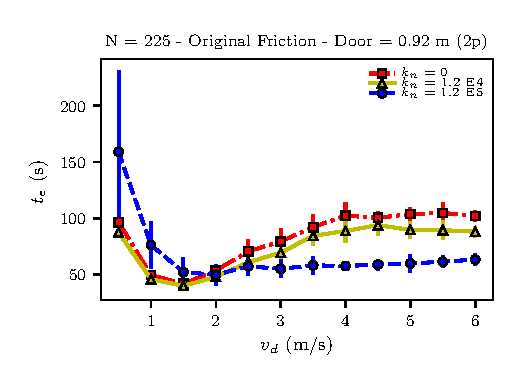
\includegraphics[width=0.7\columnwidth]
{./vd_vs_te_N225.eps}
\caption{\label{} }
\end{figure}


\begin{figure}[htbp!]
\centering
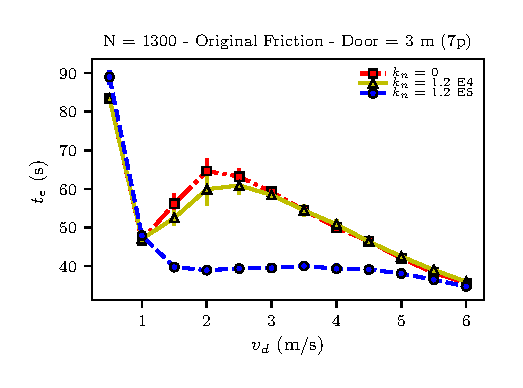
\includegraphics[width=0.7\columnwidth]
{./vd_vs_te_ck.eps}
\caption{\label{} }
\end{figure}


\begin{figure}[htbp!]
\centering
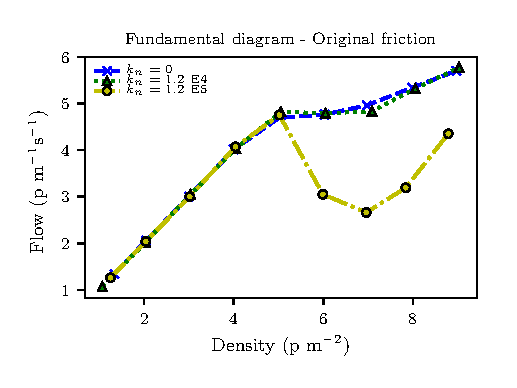
\includegraphics[width=0.7\columnwidth]
{./flow-density_vd1_multi_kn.eps}
\caption{\label{} }
\end{figure}


\begin{figure}[htbp!]
\centering
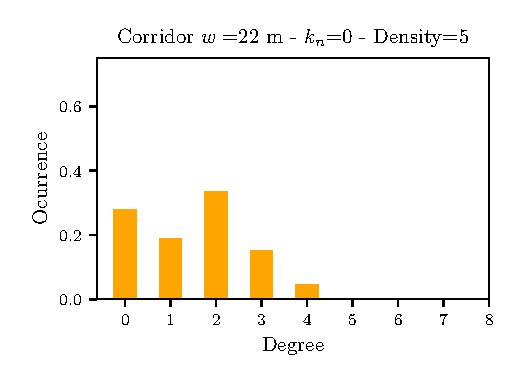
\includegraphics[width=0.7\columnwidth]
{./histo_grado_density5_width22_kn0.eps}
\caption{\label{} }
\end{figure}


\begin{figure}[htbp!]
\centering
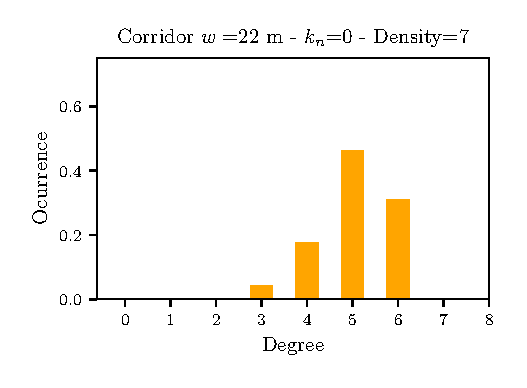
\includegraphics[width=0.7\columnwidth]
{./histo_grado_density7_width22_kn0.eps}
\caption{\label{} }
\end{figure}

\begin{figure}[htbp!]
\centering
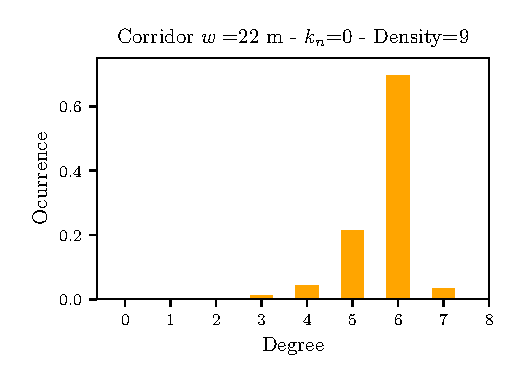
\includegraphics[width=0.7\columnwidth]
{./histo_grado_density9_width22_kn0.eps}
\caption{\label{} }
\end{figure}



\begin{figure}[htbp!]
\centering
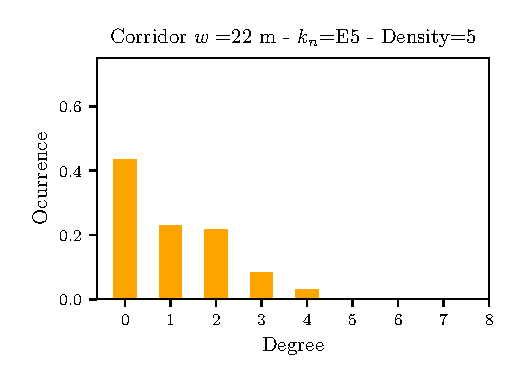
\includegraphics[width=0.7\columnwidth]
{./histo_grado_density5_width22_knE5.eps}
\caption{\label{} }
\end{figure}


\begin{figure}[htbp!]
\centering
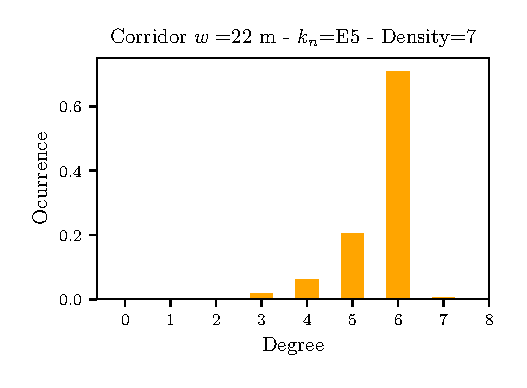
\includegraphics[width=0.7\columnwidth]
{./histo_grado_density7_width22_knE5.eps}
\caption{\label{} }
\end{figure}


\begin{figure}[htbp!]
\centering
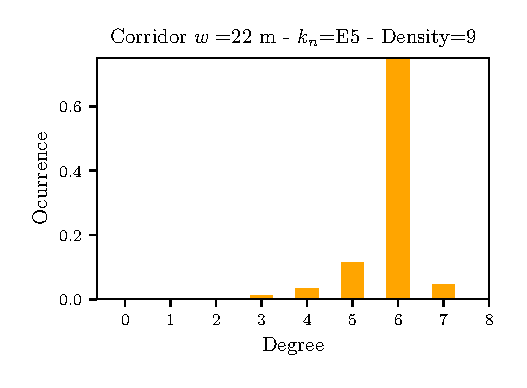
\includegraphics[width=0.7\columnwidth]
{./histo_grado_density9_width22_knE5.eps}
\caption{\label{} }
\end{figure}





\section{\label{conclusions}Conclusions}

\section*{Acknowledgments}
This work was supported by the National Scientific and Technical 
Research Council (spanish: Consejo Nacional de Investigaciones Cient\'\i ficas 
y T\'ecnicas - CONICET, Argentina) grant Programaci\'on Cient\'\i fica 2018 (UBACYT) Number 20020170100628BA.

\appendix



%/////////////////////////////////////////////////
\begin{thebibliography}{10}
\expandafter\ifx\csname url\endcsname\relax
  \def\url#1{\texttt{#1}}\fi
\expandafter\ifx\csname urlprefix\endcsname\relax\def\urlprefix{URL }\fi
\expandafter\ifx\csname href\endcsname\relax
  \def\href#1#2{#2} \def\path#1{#1}\fi

%\bibitem{helbing3}
%Helbing, D., Johansson, A., and Al-Abideen, H. Z., 2007. ``Dynamics of crowd 
%disasters: An empirical study." Physical review E 75 (4), 046109.
%{\path{https://doi.org/10.1103/PhysRevE.75.046109}}

\end{thebibliography}
\end{document}
\endinput

